\graphicspath{%
{chapter2graph/}%
{chapter2graph/bg/}}
%\makeindex


\chapter{Metrics}

\section{Variance, $\sigma^2$ or Var($X$)}

Variance is the expectation of the \underline{squared} deviation of a random variable from its \underline{mean}.  Note that the unit of variance is the square of the variable's unit. \\

1) discrete random variable\\
This is for discrete random variable (applicable to most dataset), if the generator of random variable $X$ is discrete with Probability Mass Function (PMF) that maps value $x_i$ to probability $p_i$, (certain $x_i$ and $p_i$ pairs can be same value due to same $x$ value in the dataset) then the variance will be:
\begin{eqnarray}
Var(X) = \sum_{i=1}^{n} p_i (x_i - \mu)^2
\label{variancedis}
\end{eqnarray}
where $\mu$ is the expected value:
\begin{eqnarray}
\mu = \sum_{i=1}^{n} p_i x_i
\label{expected}
\end{eqnarray}

If the each value in the $n$ data points are equally likely, then the variance will be:
\begin{eqnarray}
Var(X)= \frac{1}{n}\sum^{n}_{i=1}(x_i - \mu)^2
\label{variancediseq}
\end{eqnarray}

2) continuous random variable\\
If the random variable $X$ has a Probability Density Function (PDF) $f(x)$, then the variance will be:
\begin{eqnarray}
Var(X) = \int_{\mathbb{R}} (x - \mu)^2 f(x) dx
\label{variancecon}
\end{eqnarray}
where $\mu$ is the expected value:
\begin{eqnarray}
\mu = \int_{\mathbb{R}} xf(x)dx
\label{expectedcon}
\end{eqnarray}

\section{Standard Deviation, $\sigma$}

The standard deviation is a measure of the amount of variation or dispersion of a set of values. For both discrete and continuous random variable, the standard deviations are $\sqrt{\text{variance}}$ and note that this quantity has the same physical units as the random variable. \\

\section{Standard Error}

The standard error is a type of standard deviation for the distribution of the means. \\

There will be, of course, different means for different samples (from the same population), this is called “sampling distribution of the mean”. This variance between the means of different samples can be estimated by the standard deviation of this sampling distribution and it is the standard error of the estimate of the mean. Standard error measures the precision of the estimate of the sample mean. The standard error is strictly dependent on the sample size and thus the standard error falls as the sample size increases. It makes total sense if you think about it, the bigger the sample, the closer the sample mean is to the population mean and thus the estimate of it is closer to the actual value.
\begin{eqnarray}
\text{Standard Error} = \frac{\sigma}{\sqrt{n}}
\label{se}
\end{eqnarray}
where $\sigma$ is the standard deviation of the population (although sometimes population standard deviation is unknown, we can replace it with sample standard deviation as an estimate) and $n$ is the size (number of observations) of the sample.

\section{Confusion Matrix}

The confusion matrix is a table specifically for the problem of statistical classification. A typical confusion matrix table is shown below:

\begin{figure}[h!]
\begin{center}
	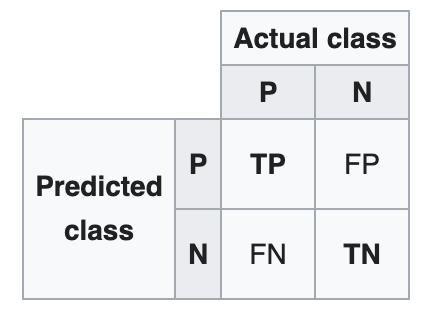
\includegraphics[scale=0.5]{confuse.png}
	\caption[]{Confusion Matrix}
	\label{confusing}
	\end{center}
	\end{figure}

where:\\
TP : True Positive or Hit \\
TN : True Negative or Correct Rejection\\
FP : False Positive or Type I error\\
FN : False Negative or Type II error\\

A more graphical way of seeing this is shown in Fig. (\ref{precisionrecall}).
\begin{figure}[h!]
\begin{center}
	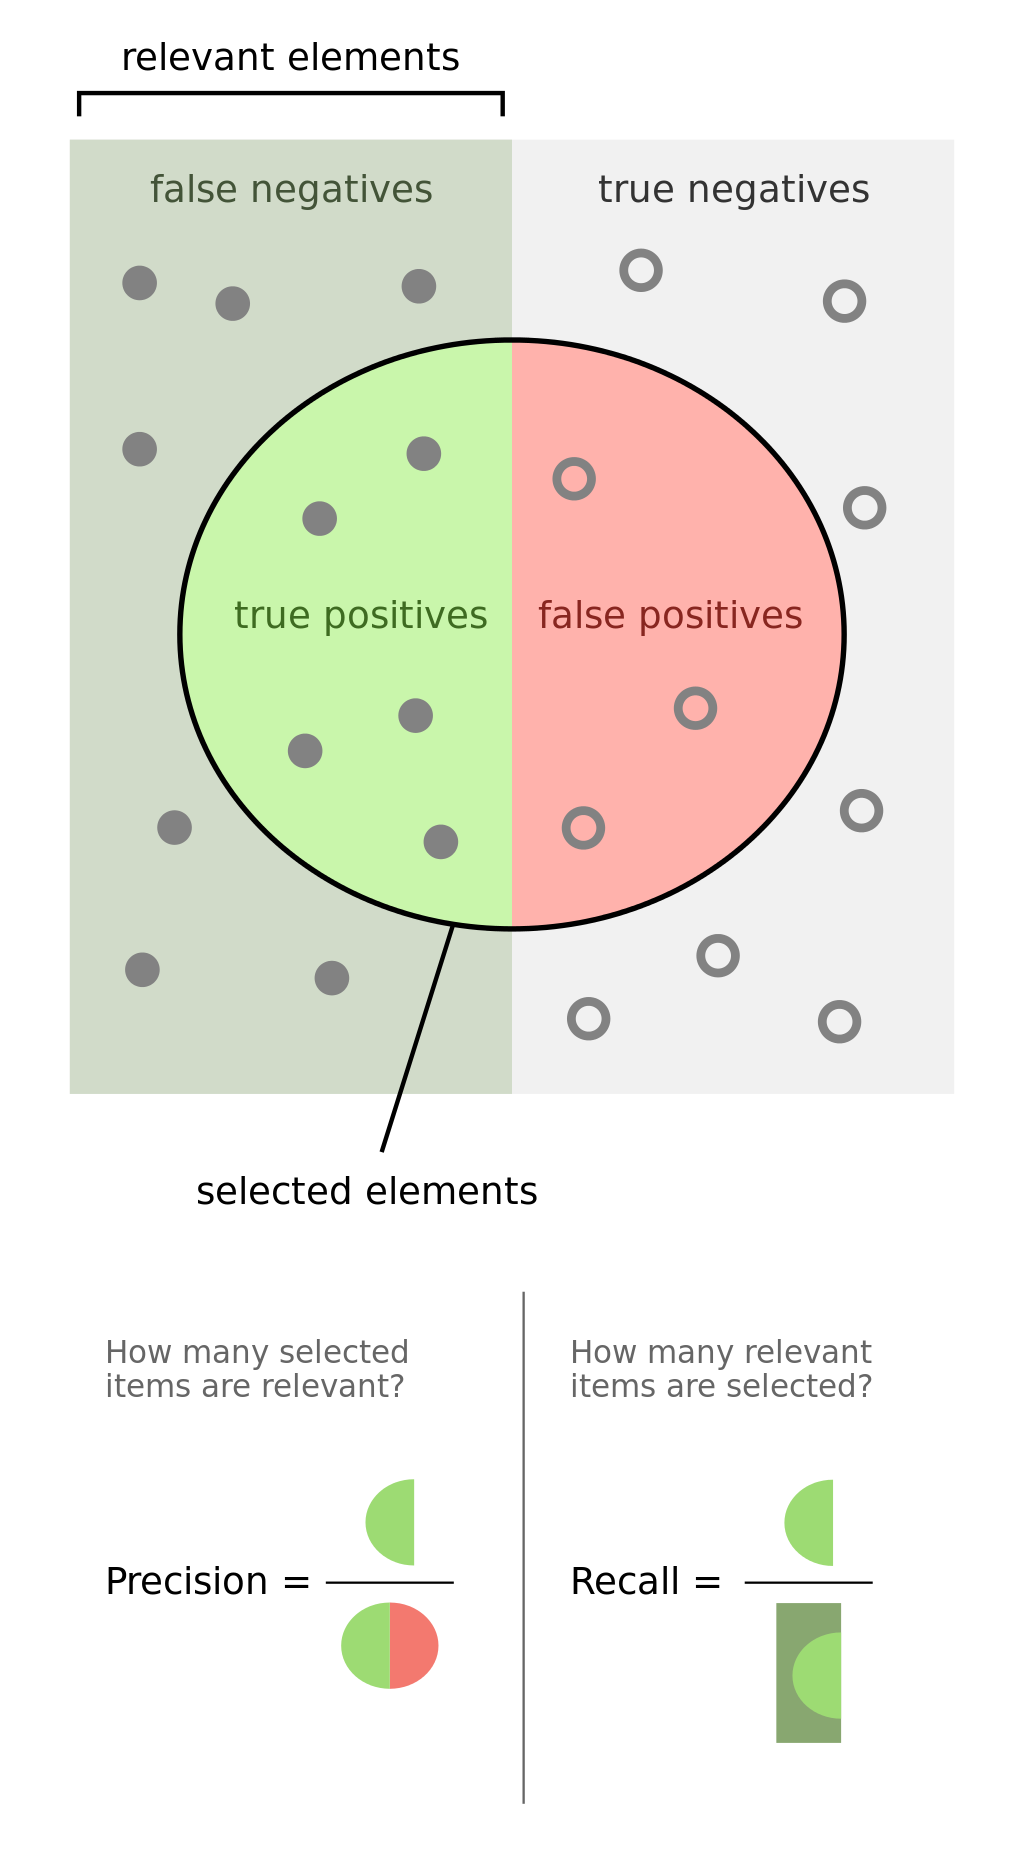
\includegraphics[scale=0.15]{precisionrecall.png}
	\caption[]{Graphical representation of confusion matrix}
	\label{precisionrecall}
	\end{center}
	\end{figure}
	
	
	
\subsection{Recall}

Recall is also called Sensitivity or True Positive Rate (TPR), it measures how many relevant items are selected (among the total numbers of relevant elements):
\begin{eqnarray}
\text{Recall} = \frac{\text{True Positive}}{\text{True Positive}+\text{False Negative}}
\label{recall}
\end{eqnarray} 

\subsection{Precision}

Precision is also called Positive Predictive Value (PPV), it measures how many selected items are relevant:
\begin{eqnarray}
\text{Precision} = \frac{\text{True Positive}}{\text{True Positive}+\text{False Positive}}
\label{precision}
\end{eqnarray} 

\subsection{$F_1$}

The $F_1$ score is a measure of a test's accuracy. It is basically the harmonic mean of the precision and recall. The highest possible $F_1$ score is 1, indicating perfect precision and recall, and the lowest possible score is 0, if either precision or recall is 0.
\begin{eqnarray}
F_1 = 2 \times \frac{\text{precision}\times\text{recall}}{\text{precision} + \text{recall}}
\label{f1}
\end{eqnarray} 

\section{ROC}



\section{Correlation/Pearson}

\section{Covariance}

\section{Confidence Interval}

\section{Confidence Level}

\section{P value}

\section{T value}

\section{Z value}




